\documentclass{standalone}

\usepackage{times}
\usepackage{amsmath}
\usepackage{amssymb}

\usepackage[dvipsnames]{xcolor}
\usepackage{tikz}
\usetikzlibrary{arrows,backgrounds,scopes}

\usepackage{pgfplots}
\pgfplotsset{compat=1.15}

%ICPC logo colors
\definecolor{red}{HTML}{972e21}
\definecolor{yellow}{HTML}{ebb83f}
\definecolor{blue}{HTML}{5e7fbf}

\begin{document}
	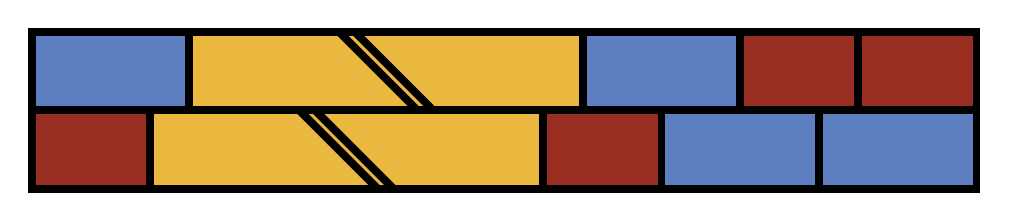
\begin{tikzpicture}[line width=0.1cm]
		\draw[fill=red] (0,0) rectangle(1.5,1);
		\draw[fill=yellow] (1.5,0) rectangle(6.5,1);
		\draw (4.4,0)--(3.4,1);
		\draw (4.6,0)--(3.6,1);
		\draw[fill=red] (6.5,0) rectangle(8,1);
		\draw[fill=blue] (8,0) rectangle(12,1);
		\draw[fill=blue] (10,0) rectangle(12,1);
		
		\draw[fill=blue] (0,1) rectangle(2,2);
		\draw[fill=yellow] (2,1) rectangle(7,2);
		\draw (4.9,1)--(3.9,2);
		\draw (5.1,1)--(4.1,2);
		\draw[fill=blue] (7,1) rectangle(9,2);
		\draw[fill=red] (9,1) rectangle(10.5,2);
		\draw[fill=red] (10.5,1) rectangle(12,2);
	\end{tikzpicture}
\end{document} 
